\documentclass[a4paper,11.5pt]{article} % тип документа


%%%Библиотеки
	%\usepackage[warn]{mathtext}	
	%\usepackage[T2A]{fontenc} % кодировка
	\usepackage[utf8]{inputenc} % кодировка исходного текста
	\usepackage[english,russian]{babel} % локализация и переносы
	\usepackage{caption}
	\usepackage{listings}
	\usepackage{amsmath,amsfonts,amssymb,amsthm,mathtools}
	\usepackage{wasysym}
	\usepackage{graphicx}%Вставка картинок правильная
	\usepackage{float}%"Плавающие" картинки
	\usepackage{wrapfig}%Обтекание фигур (таблиц, картинок и прочего)
	\usepackage{fancyhdr} %загрузим пакет
	\usepackage{lscape}
	\usepackage{xcolor}
	\usepackage[normalem]{ulem}
	\usepackage{hyperref}

%%%Конец библиотек




%%%Настройка ссылок
	\hypersetup
	{
		colorlinks=true,
		linkcolor=blue,
		filecolor=magenta,
		urlcolor=blue
	}
%%%Конец настройки ссылок


%%%Настройка колонтитулы
	\pagestyle{fancy}
	\fancyhead{}
	\fancyhead[L]{Вопрос по выбору}
	\fancyhead[R]{Талашкевич Даниил, группа Б01-009}
	\fancyfoot[C]{\thepage}
%%%конец настройки колонтитулы



							\begin{document}
						%%%%Начало документа%%%%


%%%Начало титульника
\begin{titlepage}

	\newpage
	\begin{center}
		\normalsize Московский физико-технический институт \\(госудраственный 			университет)
	\end{center}

	\vspace{6em}

	\begin{center}
		\Large Лабораторная работа по термодинамике\\
	\end{center}

	\vspace{1em}

	\begin{center}
		\large \textbf{Определение коэффициент а поверхностного натяжения жидкости [2.5.2]}
	\end{center}

	\vspace{2em}

	\begin{center}
		\large Талашкевич Даниил Александрович\\
		Группа Б01-009
	\end{center}

	\vspace{\fill}

	\begin{center}
	Долгопрудный \\2021
	\end{center}
	
\end{titlepage}
%%%Конец Титульника



%%%Настройка оглавления и нумерации страниц
	\thispagestyle{empty}
	\newpage
	\tableofcontents
	\newpage
	\setcounter{page}{1}
%%%Настройка оглавления и нумерации страниц


					%%%%%%Начало работы с текстом%%%%%%


\section{Аннотация}
\textbf{Цель работы:} 1) определение силы, необходимой для отрыва кольца от поверхности жидкости и расчет по результатам измерений коэффициента поверхностного натяжения; 2) измерение высоты подъема жидкости в капилляре и расчет его диаметра; 3) определение высоты капли жидкости на пластинке и глубины воздушного пузырька под ней; вычисление по результатам измерений
коэффициента поверхностного натяжения.\\
\textbf{В работе используются:} весы Жоли; кольцо на подвесе; штангенциркуль; грузы.

\section{Экспериментальная установка}

Установка для определения $\sigma$ (весы Жоли) изображена на (рис. 1). Тонкостенное кольцо $A$, изготовленное из материала, который  хорошо смачивается исследуемой жидкостью, подвешивается на пружине $B$. Подвеска кольца осуществляется таким образом, чтобы его ось была вертикальна. Пружина $B$ прикрепляется к кронштейну $K$, жестко связанному со штангой $\text{Б}$. Вдоль штанги $\text{Б}$ при помощи микрометрического винта $M$ передвигается столик $P$. На столике устанавливается стеклянная кювета $C$ с исследуемой жидкостью (в нашем случае с водой). Удлинение пружины $B$ (и тем самым силу ее натяжения) можно измерять по имеющейся на штанге $\text{Б}$ миллиметровой шкале.

\begin{figure}[h]
	\center{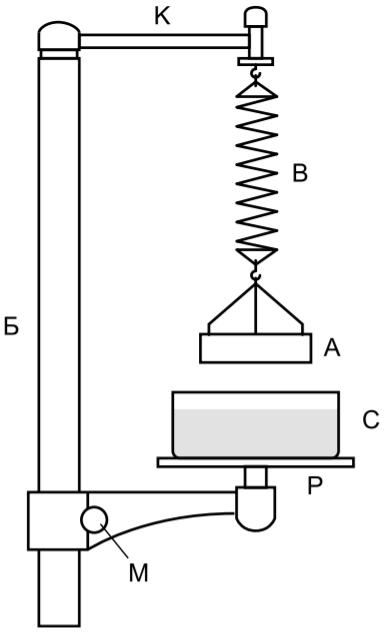
\includegraphics[scale = 0.5]{pictures/1}}
	\caption{Схема устройства весов Жоли}
	\label{pic:1}
\end{figure}

Подведем снизу кювету с водой к неподвижно висящему на пружине кольцу так, чтобы кольцо слегка коснулось поверхности воды. При этом вода начнет подниматься по стенкам кольца, а само кольцо несколько втянется внутрь жидкости. Этот эффект можно заметить по небольшому растяжению пружины в момент соприкосновения кольца с поверхностью воды.

Начнем теперь медленно опускать кювету. По мере опускания кольца пружина будет постепенно растягиваться, пока, наконец, кольцо не оторвется от поверхности воды.

В момент отрыва от воды на кольцо, кроме силы тяжести $P$, действует сила поверхностного натяжения воды $F$, которую нетрудно вычислить. «Разрежем» поверхность жидкой пленки, тянущейся из кюветы к кольцу, мысленной горизонтальной поверхностью. Нижняя часть поверхности граничит с верхней по кольцу, ограниченному двумя окружностями -- внутренней и внешней, общая длина которых близка к $4\pi R$. С помощью следующей фурмулы:
\begin{equation}
	\sigma = \frac{f}{F}.
	\label{eq:5.1}
\end{equation}
 
найдем, что сила поверхностного натяжения $F$ равна

\begin{equation}
	F = 4\pi R\sigma,
	\label{eq:1}
\end{equation}

где $R$ -- радиус кольца $A$.
 
\section{Ход работы}

\subsection{1}


\section{Вывод}
ВЫВОД

\begin{figure}[h]
%	\center{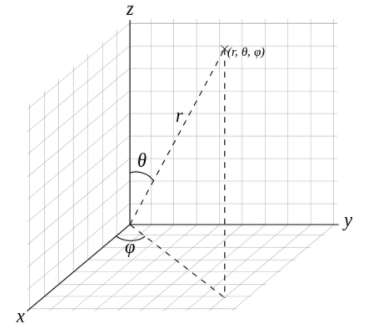
\includegraphics[scale = 0.75]{pictures/Angles}}
%	\caption{Сферическая система координат наглядно}
%	\label{Angles}
\end{figure}


					\end{document}
